%%%%%%%%%%%%%%%%%%%%%%%%%%%%%%%%%%%%%%%%%
% Beamer Presentation
% LaTeX Template
% Version 2.0 (March 8, 2022)
%
% This template originates from:
% https://www.LaTeXTemplates.com
%
% Author:
% Vel (vel@latextemplates.com)
%
% License:
% CC BY-NC-SA 4.0 (https://creativecommons.org/licenses/by-nc-sa/4.0/)
%
%%%%%%%%%%%%%%%%%%%%%%%%%%%%%%%%%%%%%%%%%

%----------------------------------------------------------------------------------------
%	PACKAGES AND OTHER DOCUMENT CONFIGURATIONS
%----------------------------------------------------------------------------------------

\documentclass[
	11pt, % Set the default font size, options include: 8pt, 9pt, 10pt, 11pt, 12pt, 14pt, 17pt, 20pt
	%t, % Uncomment to vertically align all slide content to the top of the slide, rather than the default centered
	aspectratio=169, % Uncomment to set the aspect ratio to a 16:9 ratio which matches the aspect ratio of 1080p and 4K screens and projectors
]{beamer}

%\graphicspath{{Images/}{./}} % Specifies where to look for included images (trailing slash required)

\usepackage{booktabs} % Allows the use of \toprule, \midrule and \bottomrule for better rules in tables
\usepackage{kotex}
\usepackage[backend=biber,style=authoryear]{biblatex} % 참고문헌 관련 설정
\addbibresource{references.bib} % BibTeX 파일 경로

%----------------------------------------------------------------------------------------
%	SELECT LAYOUT THEME
%----------------------------------------------------------------------------------------

% Beamer comes with a number of default layout themes which change the colors and layouts of slides. Below is a list of all themes available, uncomment each in turn to see what they look like.


\usetheme{CambridgeUS}

%----------------------------------------------------------------------------------------
%	SELECT COLOR THEME
%----------------------------------------------------------------------------------------

% Beamer comes with a number of color themes that can be applied to any layout theme to change its colors. Uncomment each of these in turn to see how they change the colors of your selected layout theme.

\usecolortheme{dolphin}

%----------------------------------------------------------------------------------------
%	SELECT FONT THEME & FONTS
%----------------------------------------------------------------------------------------

% Beamer comes with several font themes to easily change the fonts used in various parts of the presentation. Review the comments beside each one to decide if you would like to use it. Note that additional options can be specified for several of these font themes, consult the beamer documentation for more information.

\usefonttheme{default} % Typeset using the default sans serif font

%------------------------------------------------

\usepackage{mathptmx} % Use the Times font for serif text
%\usepackage{palatino} % Use the Palatino font for serif text

%\usepackage{helvet} % Use the Helvetica font for sans serif text
\usepackage[default]{opensans} % Use the Open Sans font for sans serif text
%\usepackage[default]{FiraSans} % Use the Fira Sans font for sans serif text
%\usepackage[default]{lato} % Use the Lato font for sans serif text

\usepackage[ruled,vlined]{algorithm2e}
\usepackage{algorithmicx}
\usepackage{multicol}
\usepackage{hyperref}

%----------------------------------------------------------------------------------------
%	SELECT INNER THEME
%----------------------------------------------------------------------------------------

% Inner themes change the styling of internal slide elements, for example: bullet points, blocks, bibliography entries, title pages, theorems, etc. Uncomment each theme in turn to see what changes it makes to your presentation.

%\useinnertheme{default}
\useinnertheme{circles}

%----------------------------------------------------------------------------------------
%	Other Change
%----------------------------------------------------------------------------------------

% Change standard block width
\addtobeamertemplate{block begin}{%
    \setlength{\textwidth}{0.9\textwidth}
}{}


%----------------------------------------------------------------------------------------
%	PRESENTATION INFORMATION
%----------------------------------------------------------------------------------------

\title[OPF using Matpower and Pyomo]{Multi Period Optimal Power Flow \\ using Matpower and Pyomo} % The short title in the optional parameter appears at the bottom of every slide, the full title in the main parameter is only on the title page

%\subtitle{Optional Subtitle} % Presentation subtitle, remove this command if a subtitle isn't required

\author[Taeho Nam]{Taeho Nam} % Presenter name(s), the optional parameter can contain a shortened version to appear on the bottom of every slide, while the main parameter will appear on the title slide

\institute[CWNU]{Changwon National University \\ \smallskip \textit{rapitransit@gmail.com}} % Your institution, the optional parameter can be used for the institution shorthand and will appear on the bottom of every slide after author names, while the required parameter is used on the title slide and can include your email address or additional information on separate lines

\date[\today]{\today} % Presentation date or conference/meeting name, the optional parameter can contain a shortened version to appear on the bottom of every slide, while the required parameter value is output to the title slide

%----------------------------------------------------------------------------------------

\begin{document}

%----------------------------------------------------------------------------------------
%	TITLE SLIDE
%----------------------------------------------------------------------------------------

\begin{frame}
	\titlepage % Output the title slide, automatically created using the text entered in the PRESENTATION INFORMATION block above
\end{frame}

%----------------------------------------------------------------------------------------
%	TABLE OF CONTENTS SLIDE
%----------------------------------------------------------------------------------------

% The table of contents outputs the sections and subsections that appear in your presentation, specified with the standard \section and \subsection commands. You may either display all sections and subsections on one slide with \tableofcontents, or display each section at a time on subsequent slides with \tableofcontents[pausesections]. The latter is useful if you want to step through each section and mention what you will discuss.

\begin{frame}[allowframebreaks]
	\frametitle{Table of Contents} % Slide title, remove this command for no title
	
	\tableofcontents % Output the table of contents (all sections on one slide)
	%\tableofcontents[pausesections] % Output the table of contents (break sections up across separate slides)
\end{frame}

%----------------------------------------------------------------------------------------
%	PRESENTATION BODY SLIDES
%----------------------------------------------------------------------------------------

%------------------------------------------------
\section{Background}

\begin{frame}
    \centering
    \LARGE
    Background
\end{frame}
%------------------------------------------------
\subsection{Multi Period Optimal Power Flow(MPOPF)}

\begin{frame}
	\frametitle{Multi Period Optimal Power Flow}

	\begin{itemize}
		\item \textbf{MPOPF} (Multi-Period Optimal Power Flow) is a method for optimizing the operation of a power system over multiple time periods.
		\item It extends the conventional single-period Optimal Power Flow (OPF) to consider multiple time intervals.
	\end{itemize}

	\begin{figure}
		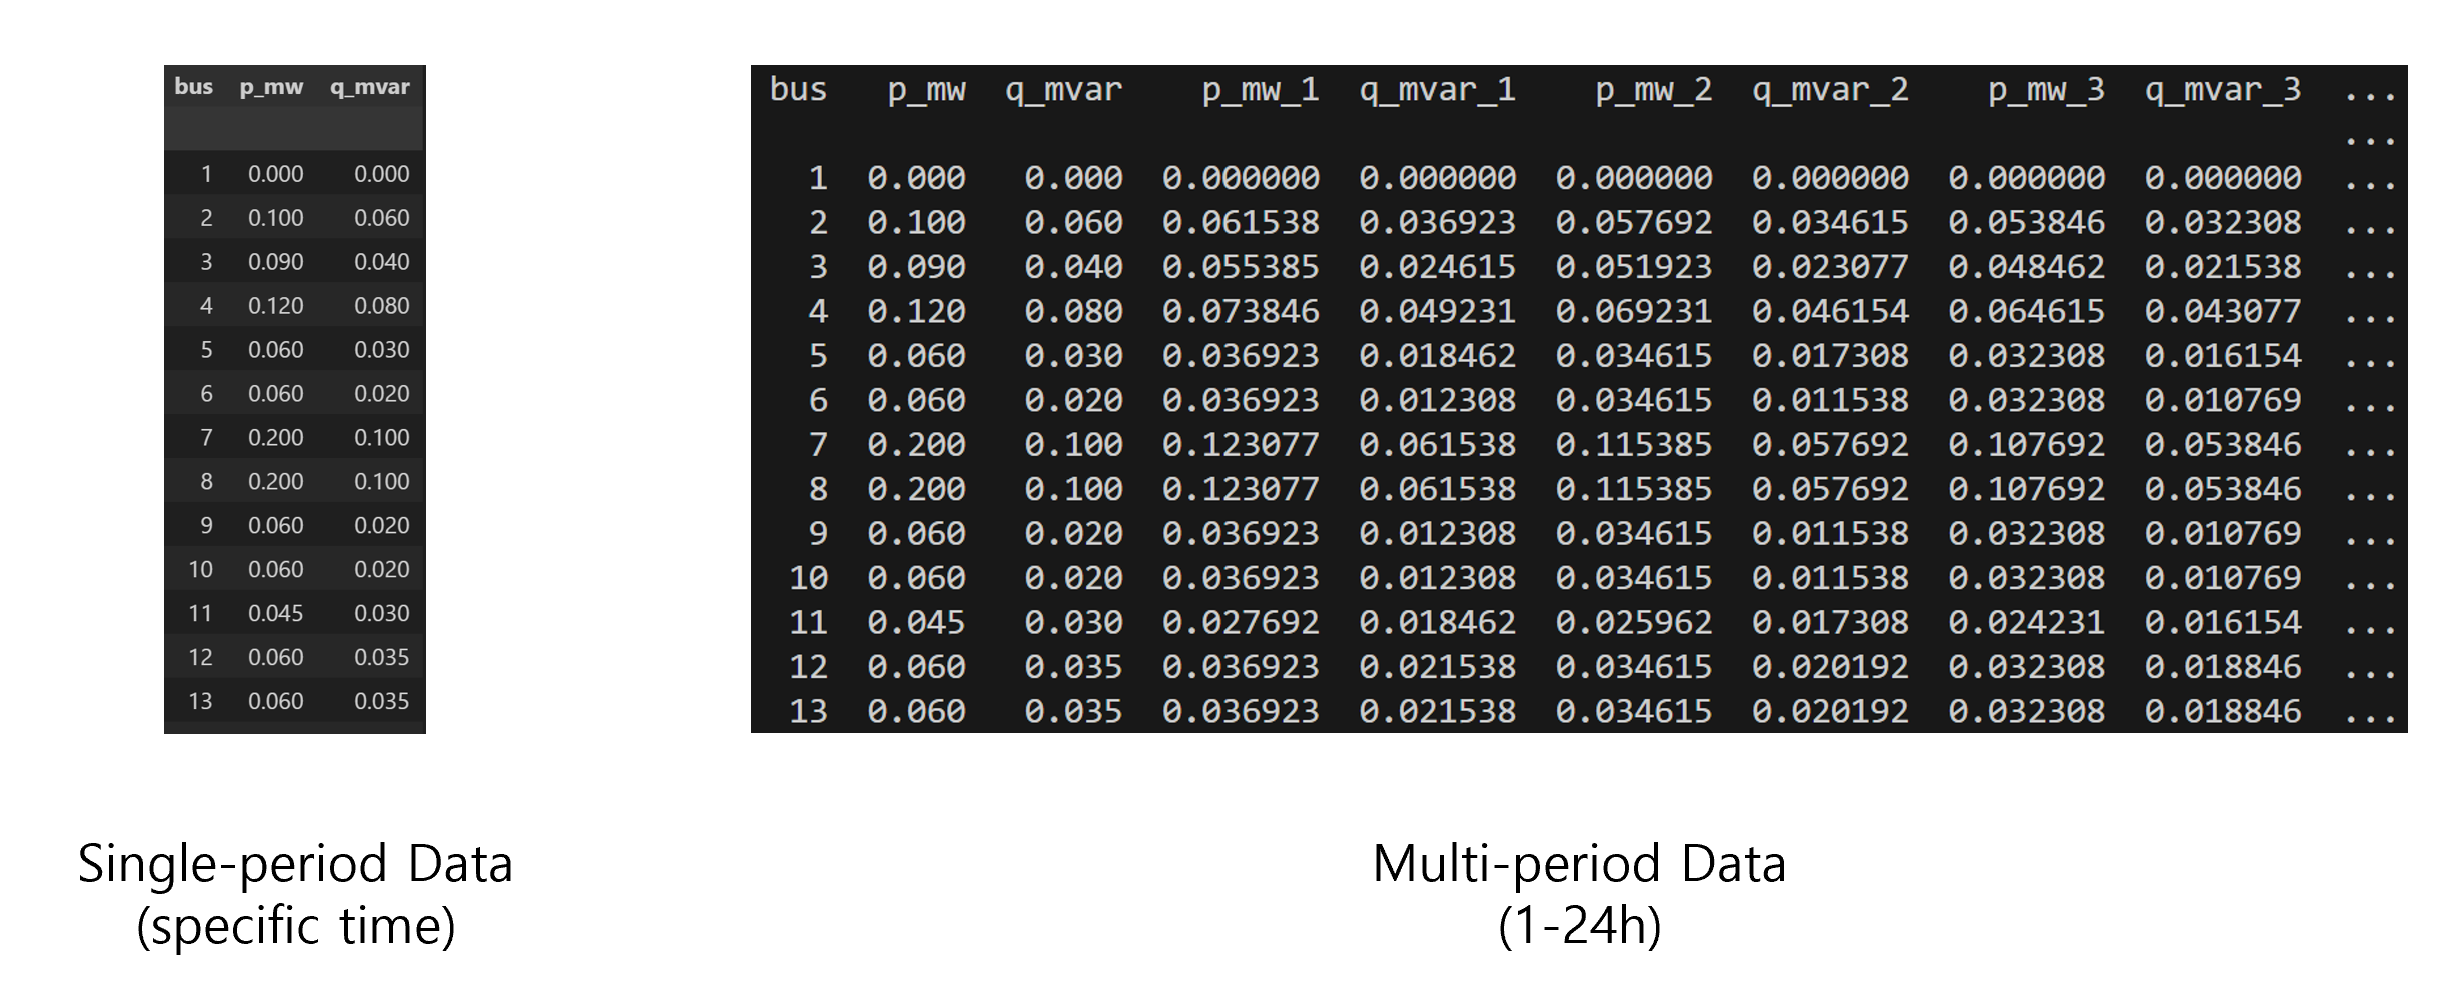
\includegraphics[width=4 in,keepaspectratio]{MPOPFtime.png}
	\end{figure}
	
\end{frame}

% %------------------------------------------------
% \subsection{Reconfiguragble Distribution System}

% \begin{frame}
% 	\frametitle{Reconfiguragble Distribution System}
	
% 	\begin{itemize}
% 		\item \textbf{Reconfigurable Distribution System} is an electrical power distribution network that can dynamically change its structure or topology.
% 		\item This is achieved by remotely opening and closing sectionalizing and tie switches within the network.
% 	\end{itemize}

% 	\begin{figure}
% 		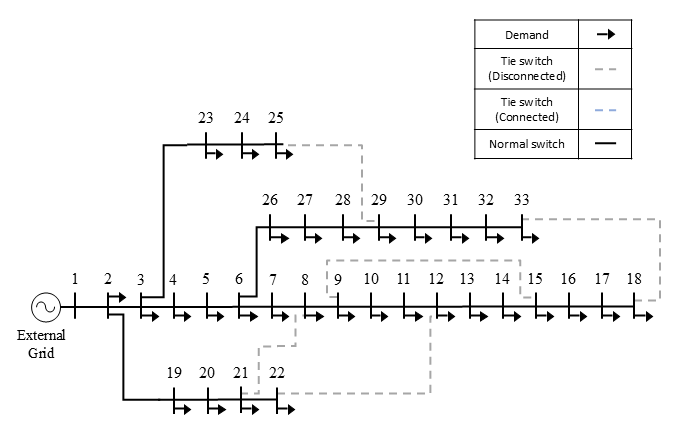
\includegraphics[width=3 in,keepaspectratio]{modified_33_bus.png}
% 	\end{figure}

% \end{frame}

%------------------------------------------------
\section{MPOPF Flow Formulation} % Sections are added in order to organize your presentation into discrete blocks, all sections and subsections are automatically output to the table of contents as an overview of the talk but NOT output in the presentation as separate slides

\begin{frame}
    \centering
    \LARGE
    Multi Period Optimal Power Flow Formulation
\end{frame}

%------------------------------------------------

\subsection{MPOPF Overview}

\begin{frame}
	\frametitle{Overview}
	
	\begin{columns}
		\begin{column}{0.5\textwidth}
			\begin{itemize}
				\item MPOPF Nomenclature: Slide~\ref{frame:MPOFP_nomenclature}
				\item MPOPF At glance...: Slide~\ref{frame:MPOFP_atglance}
				\item MPOPF Objective function: Slide~\ref{frame:MPOFP_objfunc}
				\item MPOPF Constraints and expressions: Slide~\ref{frame:MPOFP_constraints}
					\begin{itemize}
						\item MPOPF Load balance
						\item MPOPF Power and voltage
						\item MPOPF Current
					\end{itemize}
			\end{itemize}
		\end{column}

		\begin{column}{0.5\textwidth}
			Optimization problem is formulated as:
			\begin{enumerate}
				\item MPOPF Objective function:
				\[
					\text{minimize (or maximize) } f(\mathbf{x})
				\]
				\item MPOPF Constraints:
				\[
					g(\mathbf{x}) \leq 0, \quad h(\mathbf{x}) = 0
				\]
				\item MPOPF Functions in the objective and constraints:
				\[
					f(\mathbf{x}), \quad g(\mathbf{x}), \quad h(\mathbf{x})
				\]
			\end{enumerate}
		\end{column}
	\end{columns}
\end{frame}

%------------------------------------------------

\subsection{Nomenclature}

\begin{frame}

	\frametitle{Nomenclature}
	\label{frame:MPOFP_nomenclature}
	\framesubtitle{Sets, indices, parameters}
	
	\begin{columns}
	
		\begin{column}{0.5\textwidth}
			
			\begin{itemize}
			\item Indices
			\end{itemize}

			\begin{tabular}{ll}
				$i,j$ & Index of bus \\
				$l$ & Index of line \\
				$t$ & Index of time \\
			\end{tabular}

		\end{column}

		\begin{column}{0.5\textwidth}
			
			\begin{itemize}
			\item Sets
			\end{itemize}

			\begin{tabular}{ll}
				$\Omega_{l}$ & Set of lines \\
				$\Omega_{b}$ & Set of buses\\
				$\Omega_{b_{i}}$ & \begin{tabular}[l]{@{}l@{}}Set of connected buses \\ in the bus $i$\end{tabular}\\
				$\Omega_{b_{g}}$ & \begin{tabular}[l]{@{}l@{}}Set of generation buses \\ ($\Omega_{b_{g}}$ $\subset$ $\Omega_{b}$)\end{tabular}\\
				$T$ & \begin{tabular}[l]{@{}l@{}}The total time period\\ (e.g 1,2...,24 for 24 hours)\end{tabular}\\
			\end{tabular}

		\end{column}


	\end{columns}

\end{frame}

%------------------------------------------------

\begin{frame}
	\frametitle{Nomenclature}
	\framesubtitle{Sets, indices, parameters}

	\begin{columns}
		\begin{column}{0.5\textwidth}
			\begin{itemize}
			\item Parameters or constants
			\end{itemize}

			\begin{tabular}{ll}
				$Z_{ij}$, $Y_{ij}$ & \begin{tabular}[l]{@{}l@{}}Impedance and \\admittance of line $ij$\\(from bus $i$ to bus $j$)\end{tabular} \\
				$G_{ij}$, $B_{ij}$ & \begin{tabular}[l]{@{}l@{}}Conductance and \\susceptance of line $ij$\\(from bus $i$ to bus $j$)\end{tabular} \\
				$\overline{V}$, $\underline{V}$ & \begin{tabular}[l]{@{}l@{}}Maximum and minimum \\voltage magnitude\end{tabular}\\
				$\overline{I}_{ij}$ & \begin{tabular}[l]{@{}l@{}}Maximum current \\ flow limit of line $ij$\end{tabular}\\
			\end{tabular}
		\end{column}

		\begin{column}{0.5\textwidth}
			\begin{tabular}{ll}
				$P_{D_{i,t}}$, $Q_{D_{i,t}}$ & \begin{tabular}[l]{@{}l@{}}Active and reactive \\ power demand at bus $i$\end{tabular}\\
				$\overline{P}_{G_{i}}$, $\underline{P}_{G_{i}}$ & \begin{tabular}[l]{@{}l@{}}Maximum and minimum \\active power from generator \\ at bus $i$\end{tabular}\\
				$\overline{Q}_{G_{i}}$, $\underline{Q}_{G_{i}}$ & \begin{tabular}[l]{@{}l@{}}Maximum and minimum \\reactive power from \\ generator at bus $i$\end{tabular}\\
				$baseMVA$ & Value of base MVA \\
			\end{tabular}
		\end{column}
	\end{columns}

\end{frame}

%------------------------------------------------

\begin{frame}
	\frametitle{Nomenclature}
	\framesubtitle{Sets, indices, parameters}

	\begin{columns}
		\begin{column}{0.5\textwidth}
			\begin{itemize}
			\item Functions
			\end{itemize}

			\begin{tabular}{ll}
				$P_{ij,t}$, $Q_{ij,t}$& \begin{tabular}[l]{@{}l@{}}Active and reactive power \\ flow of line $ij$ at time $t$\end{tabular}\\
				$I_{r_{ij,t}}$, $I_{Im_{ij,t}}$& \begin{tabular}[l]{@{}l@{}}Real and Imaginary current \\ flow of line $ij$ at time $t$\end{tabular}\\
				$P^{lineloss}_{l,t}$& \begin{tabular}[l]{@{}l@{}}Active line loss of line $l(ij)$ \\ at time $t$\end{tabular}\\
			\end{tabular}
		\end{column}

		\begin{column}{0.5\textwidth}
			\begin{itemize}
			\item Variables
			\end{itemize}

			\begin{tabular}{ll}
				$\left|\dot{V}_{i,t} \right|$ & \begin{tabular}[l]{@{}l@{}} Voltage magnitude in bus $i$ \\ at time $t$ \\ \end{tabular}\\
				$\theta_{i,t}$ & \begin{tabular}[l]{@{}l@{}}Voltage phase angle in bus $i$ \\ at time $t$ \\ \end{tabular}\\
				$P_{G_{i,t}}$, $Q_{G_{i,t}}$ & \begin{tabular}[l]{@{}l@{}}Active and reactive power \\from generator at bus $i$ \\ at time $t$ \end{tabular}\\
			\end{tabular}

		\end{column}

	\end{columns}

\end{frame}

%------------------------------------------------

\subsection{MPOPF At glance...}

\begin{frame}
	\frametitle{MPOPF At glance...}
	\label{frame:MPOFP_atglance}
	
	Objective function: Eq.~\eqref{eq:Mobj}
	\begin{align*}
		\min{ \sum_{\forall t} \sum_{\forall i,j} {[-G_{ij}(\left|\dot{V}_{i,t} \right|^2 + \left|\dot{V}_{j,t} \right|^2) + 2G_{ij}\left|\dot{V}_{i,t} \right|\left|\dot{V}_{j,t} \right|\cos\left(\theta_{i,t}-\theta_{j,t} \right) ]} }
	\end{align*}

	Constraints: Eqs.~\eqref{eq:Mcons_load_bal_P},\eqref{eq:Mcons_load_bal_Q},\eqref{eq:Mcons_power_P},\eqref{eq:Mcons_power_Q},\eqref{eq:Mcons_voltage},\eqref{eq:Mcons_slack},\eqref{eq:Mcons_current}

	\vspace{-0.5em}
	\begin{columns}
		\begin{column}{0.5\textwidth}
			\begin{align*}
				P_{G_{i,t}} - P_{D_{i,t}} = \sum_{j \in \Omega_{b_{i}}}(P_{ij,t})  \quad \forall i \in \Omega_{b},\ \forall t \in T\\
				Q_{G_{i,t}} - Q_{D_{i,t}} = \sum_{j \in \Omega_{b_{i}}}(Q_{ij,t})  \quad \forall i \in \Omega_{b},\ \forall t \in T\\
				\underline{P}_{G_{i}} \leq P_{G_{i,t}} \leq \overline{P}_{G_{i}} \quad \forall i \in \Omega_{b},\ \forall t \in T\\
				\underline{Q}_{G_{i}} \leq Q_{G_{i,t}} \leq \overline{Q}_{G_{i}}  \quad \forall i \in \Omega_{b},\ \forall t \in T\\
			\end{align*}
		\end{column}

		\begin{column}{0.5\textwidth}
			\begin{align*}
				\underline{V} \leq \left|\dot{V}_{i,t} \right| \leq \overline{V}  \quad \forall i \in \Omega_{b},\ \forall t \in T\\
				\theta_{i,t} = \left\{ \begin{array}{cl}
							0 & : \ \text{Bus } i \text{ is slack,} \\
							\text{free} & : \ \text{Otherwise.}
							\end{array} \right.\\
				I_{r_{ij,t}}^{2}+ I_{Im_{ij,t}}^{2} \leq \overline{I}_{ij}^{2} \quad   \forall l(ij) \in \Omega_{l},\ \forall t \in T\\
			\end{align*}
		\end{column}
	\end{columns}
	
\end{frame}

%------------------------------------------------

\begin{frame}
	\frametitle{MPOPF At glance...}

	Functions or expressions: Eq.~\eqref{eq:Mexpr_loss}, \eqref{eq:Mexpr_p_flow_ij}, \eqref{eq:Mexpr_p_flow_ji}

	\begin{gather*}
		[-G_{ij}(\left|\dot{V}_{i,t} \right|^2 + \left|\dot{V}_{j,t} \right|^2) + 2G_{ij}\left|\dot{V}_{i,t} \right|\left|\dot{V}_{j,t} \right|\cos\left(\theta_{i,t}-\theta_{j,t} \right) ] \\
		= P_{l,t}^{line loss} = P_{ij,t} + P_{ji,t} \\[1em]
		\forall l(ij) \in \Omega_{l},\ \forall t \in T
	\end{gather*}

	
\end{frame}

%------------------------------------------------

\begin{frame}
	\frametitle{MPOPF At glance...}

	\begin{gather*}
		\begin{aligned}
			P_{ij,t} =\ &-G_{ij} \left|\dot{V}_{i,t} \right|^2 
			+ G_{ij} \left|\dot{V}_{i,t} \right| \left|\dot{V}_{j,t} \right| \cos\left(\theta_{i,t}-\theta_{j,t} \right) \\
			&+ B_{ij} \left|\dot{V}_{i,t} \right| \left|\dot{V}_{j,t} \right| \sin\left(\theta_{i,t}-\theta_{j,t} \right) \\[1em]
			&\qquad \forall l(ij) \in \Omega_{l},\ \forall t \in T
		\end{aligned}
		\\[2em]
		\begin{aligned}
			P_{ji,t} =\ &-G_{ij} \left|\dot{V}_{j,t} \right|^2 
			+ G_{ij} \left|\dot{V}_{i,t} \right| \left|\dot{V}_{j,t} \right| \cos\left(\theta_{i,t}-\theta_{j,t} \right) \\
			&- B_{ij} \left|\dot{V}_{i,t} \right| \left|\dot{V}_{j,t} \right| \sin\left(\theta_{i,t}-\theta_{j,t} \right) \\[1em]
			&\qquad \forall l(ij) \in \Omega_{l},\ \forall t \in T
		\end{aligned}
	\end{gather*}


	
\end{frame}

%------------------------------------------------
\begin{frame}
	\frametitle{MPOPF At Glance}
	
	Functions or expressions (Continued): Eq.~\eqref{eq:Mexpr_q_flow_ij},\eqref{eq:Mexpr_q_flow_ji}, \eqref{eq:Mexpr_i_re}, \eqref{eq:Mexpr_i_imag}
	
	\begin{align*}
		\begin{split}
			Q_{ij,t} =&\ B_{ij}\left\lvert \dot{V}_{i,t}\right\rvert^{2} + G_{ij}\left\lvert \dot{V}_{i,t}\right\rvert\left\lvert \dot{V}_{j,t}\right\rvert \sin{\left(\theta_{i,t}-\theta_{j,t}\right)} \\
			&- B_{ij}\left\lvert \dot{V}_{i,t}\right\rvert\left\lvert \dot{V}_{j,t}\right\rvert \cos{\left(\theta_{i,t}-\theta_{j,t}\right)}  \\[1em]
			&\qquad \forall l(ij) \in \Omega_{l},\ \forall t \in T
		\end{split}
	\end{align*}

	\begin{align*}
		\begin{split}
			Q_{ji,t} =&\ B_{ij}\left\lvert \dot{V}_{j,t}\right\rvert^{2} - G_{ij}\left\lvert \dot{V}_{i,t}\right\rvert\left\lvert \dot{V}_{j,t}\right\rvert \sin{\left(\theta_{i,t}-\theta_{j,t}\right)} \\
			&- B_{ij}\left\lvert \dot{V}_{i,t}\right\rvert\left\lvert \dot{V}_{j,t}\right\rvert \cos{\left(\theta_{i,t}-\theta_{j,t}\right)}  \\[1em]
			&\qquad \forall l(ij) \in \Omega_{l},\ \forall t \in T
		\end{split}
	\end{align*}
	

\end{frame}


%------------------------------------------------

\begin{frame}
	\frametitle{MPOPF At Glance}
	
	\begin{align*}
		\begin{split}
			I_{r_{ij,t}} = &-G_{ij}\left\lvert \dot{V}_{i,t} \right\rvert \cos{\theta_{i,t}} + B_{ij}\left\lvert \dot{V}_{i,t} \right\rvert \sin{\theta_{i,t}} \\
					&+ G_{ij}\left\lvert \dot{V}_{j,t} \right\rvert \cos{\theta_{j,t}} - B_{ij}\left\lvert \dot{V}_{j,t} \right\rvert \sin{\theta_{j,t}} \\[1em]
			&\qquad \forall l(ij) \in \Omega_{l},\ \forall t \in T
		\end{split}
	\end{align*}

	\begin{align*}
		\begin{split}
			I_{Im_{ij,t}} = &-B_{ij}\left\lvert \dot{V}_{i,t} \right\rvert \cos{\theta_{i,t}} - G_{ij}\left\lvert \dot{V}_{i,t} \right\rvert \sin{\theta_{i,t}} \\
			&+ B_{ij}\left\lvert \dot{V}_{j,t} \right\rvert \cos{\theta_{j,t}} + G_{ij}\left\lvert \dot{V}_{j,t} \right\rvert \sin{\theta_{j,t}} \\[1em]
			&\qquad \forall l(ij) \in \Omega_{l},\ \forall t \in T
		\end{split}
	\end{align*}

\end{frame}
%------------------------------------------------

\subsection{Objective function}

\begin{frame}
	\frametitle{Objective function}
	\label{frame:MPOFP_objfunc}

    \begin{equation}
    \label{eq:Mobj}
        \min \sum_{\forall t} \sum_{\forall i,j} \Big[ -G_{ij}\big(\left|\dot{V}_{i,t}\right|^2 + \left|\dot{V}_{j,t}\right|^2\big) + 2G_{ij}\left|\dot{V}_{i,t}\right|\left|\dot{V}_{j,t}\right|\cos\big(\theta_{i,t}-\theta_{j,t}\big) \Big]
    \end{equation}

	\vspace{1.5em}

	\begin{equation}
    \label{eq:Mexpr_loss}
        \begin{gathered}
            \Big[ -G_{ij}\big(\left|\dot{V}_{i,t}\right|^2 + \left|\dot{V}_{j,t}\right|^2\big) + 2G_{ij}\left|\dot{V}_{i,t}\right|\left|\dot{V}_{j,t}\right|\cos\big(\theta_{i,t}-\theta_{j,t}\big) \Big] = P_{l,t}^{line loss} = P_{ij,t} + P_{ji,t} \\[1em]
            \forall l(ij) \in \Omega_{l},\ \forall t \in T
        \end{gathered}
    \end{equation}

\end{frame}

%------------------------------------------------

\begin{frame}
	\frametitle{MPOPF Objective function}

	\begin{align}
	\label{eq:Mexpr_p_flow_ij}
		\begin{split}
		P_{ij,t} =\ &-G_{ij} \left|\dot{V}_{i,t}\right|^2 
		+ G_{ij} \left|\dot{V}_{i,t}\right|\left|\dot{V}_{j,t}\right| \cos\big(\theta_{i,t}-\theta_{j,t}\big) \\
		&+ B_{ij} \left|\dot{V}_{i,t}\right|\left|\dot{V}_{j,t}\right| \sin\big(\theta_{i,t}-\theta_{j,t}\big) \\[1em]
		&\qquad \forall l(ij) \in \Omega_{l},\ \forall t \in T
		\end{split}
	\end{align}

	\begin{align}
	\label{eq:Mexpr_p_flow_ji}
		\begin{split}
		P_{ji,t} =\ &-G_{ij} \left|\dot{V}_{j,t}\right|^2 
		+ G_{ij} \left|\dot{V}_{i,t}\right|\left|\dot{V}_{j,t}\right| \cos\big(\theta_{i,t}-\theta_{j,t}\big) \\
		&- B_{ij} \left|\dot{V}_{i,t}\right|\left|\dot{V}_{j,t}\right| \sin\big(\theta_{i,t}-\theta_{j,t}\big) \\[1em]
		&\qquad \forall l(ij) \in \Omega_{l},\ \forall t \in T
		\end{split}
	\end{align}

\end{frame}

%------------------------------------------------

\subsection{Constraints}

\begin{frame}
	\frametitle{MPOPF Constraints}
	\label{frame:MPOFP_constraints}
	\framesubtitle{Load balance} % Optional subtitle

	\begin{align}
	\label{eq:Mcons_load_bal_P}
		P_{G_{i,t}} - P_{D_{i,t}} = \sum_{j \in \Omega_{b_{i}}} P_{ij,t}  \quad \forall i \in \Omega_{b},\ \forall t \in T
	\end{align}

	\begin{align}
	\label{eq:Mcons_load_bal_Q}
		Q_{G_{i,t}} - Q_{D_{i,t}} = \sum_{j \in \Omega_{b_{i}}} Q_{ij,t}  \quad \forall i \in \Omega_{b},\ \forall t \in T
	\end{align}

\end{frame}

%------------------------------------------------


\begin{frame}
	\frametitle{MPOPF Constraints}
	\framesubtitle{Load balance} % Optional subtitle

	\begin{align}
	\label{eq:Mexpr_q_flow_ij}
		\begin{split}
			Q_{ij,t} =\ &B_{ij}\left\lvert \dot{V}_{i,t}\right\rvert^{2} + G_{ij}\left\lvert \dot{V}_{i,t}\right\rvert\left\lvert \dot{V}_{j,t}\right\rvert \sin{\left(\theta_{i,t}-\theta_{j,t}\right)} \\
			&- B_{ij}\left\lvert \dot{V}_{i,t}\right\rvert\left\lvert \dot{V}_{j,t}\right\rvert \cos{\left(\theta_{i,t}-\theta_{j,t}\right)} \\[1em]
			&\qquad \forall l(ij) \in \Omega_{l},\ \forall t \in T
		\end{split}
	\end{align}

	\begin{align}
	\label{eq:Mexpr_q_flow_ji}
		\begin{split}
			Q_{ji,t} =\ &B_{ij}\left\lvert \dot{V}_{j,t}\right\rvert^{2} - G_{ij}\left\lvert \dot{V}_{i,t}\right\rvert\left\lvert \dot{V}_{j,t}\right\rvert \sin{\left(\theta_{i,t}-\theta_{j,t}\right)} \\
			&- B_{ij}\left\lvert \dot{V}_{i,t}\right\rvert\left\lvert \dot{V}_{j,t}\right\rvert \cos{\left(\theta_{i,t}-\theta_{j,t}\right)} \\[1em]
			&\qquad \forall l(ij) \in \Omega_{l},\ \forall t \in T
		\end{split}
\end{align}

\end{frame}

%------------------------------------------------

\begin{frame}
	\frametitle{MPOPF Constraints}
	\framesubtitle{Power and voltage} % Optional subtitle

	\vspace{-1.2em}

	\begin{align}
	\label{eq:Mcons_power_P}
		\underline{P}_{G_{i}} \leq P_{G_{i,t}} \leq \overline{P}_{G_{i}}  \quad \forall i \in \Omega_{b},\ \forall t \in T
	\end{align}

	\begin{align}
	\label{eq:Mcons_power_Q}
		\underline{Q}_{G_{i}} \leq Q_{G_{i,t}} \leq \overline{Q}_{G_{i}}  \quad \forall i \in \Omega_{b},\ \forall t \in T
	\end{align}

	\begin{align}
	\label{eq:Mcons_voltage}
		\underline{V} \leq \left|\dot{V}_{i,t} \right| \leq \overline{V}  \quad \forall i \in \Omega_{b},\ \forall t \in T
	\end{align}

	\begin{align}
	\label{eq:Mcons_slack}
		\theta_{i,t} = \left\{ \begin{array}{cl}
							0 & : \ \text{Bus } i \text{ is slack,} \\
							\text{free} & : \ \text{Otherwise.}
							\end{array} \right. \quad \forall t \in T
	\end{align}

	\begin{align}
	\label{eq:Mcons_current}
		I_{r_{ij,t}}^{2}+ I_{Im_{ij,t}}^{2} \leq \overline{I}_{ij}^{2} \quad   \forall l(ij) \in \Omega_{l},\ \forall t \in T
	\end{align}


\end{frame}

%------------------------------------------------

\begin{frame}
	\frametitle{MPOPF Constraints}
	\framesubtitle{Current} % Optional subtitle

	\begin{align}
	\label{eq:Mexpr_i_re}
		\begin{split}
			I_{r_{ij,t}} =\ &-G_{ij}\left\lvert \dot{V}_{i,t} \right\rvert \cos{\theta_{i,t}} + B_{ij}\left\lvert \dot{V}_{i,t} \right\rvert \sin{\theta_{i,t}} \\
					&+ G_{ij}\left\lvert \dot{V}_{j,t} \right\rvert \cos{\theta_{j,t}} - B_{ij}\left\lvert \dot{V}_{j,t} \right\rvert \sin{\theta_{j,t}} \\[1em]
			&\qquad \forall l(ij) \in \Omega_{l},\  \forall t \in T
		\end{split}
	\end{align}

	\begin{align}
	\label{eq:Mexpr_i_imag}
		\begin{split}
			I_{Im_{ij,t}} =\ &-B_{ij}\left\lvert \dot{V}_{i,t} \right\rvert \cos{\theta_{i,t}} - G_{ij}\left\lvert \dot{V}_{i,t} \right\rvert \sin{\theta_{i,t}} \\
			&+ B_{ij}\left\lvert \dot{V}_{j,t} \right\rvert \cos{\theta_{j,t}} + G_{ij}\left\lvert \dot{V}_{j,t} \right\rvert \sin{\theta_{j,t}} \\[1em]
			&\qquad \forall l(ij) \in \Omega_{l},\ \forall t \in T
		\end{split}
	\end{align}

\end{frame}
	
%------------------------------------------------

\section{Implementation of MPOPF in a 33-bus distribution system}

\begin{frame}
    \centering
    \LARGE
    Implementation of Multi-Period Optimal Power Flow \\ in a 33-bus distribution system
\end{frame}

%------------------------------------------------

\subsection{33-bus distribution system}


\begin{frame}
	\frametitle{33-bus distribution system}
	\framesubtitle{Structure of the 33-bus distribution system}

	\begin{figure}
		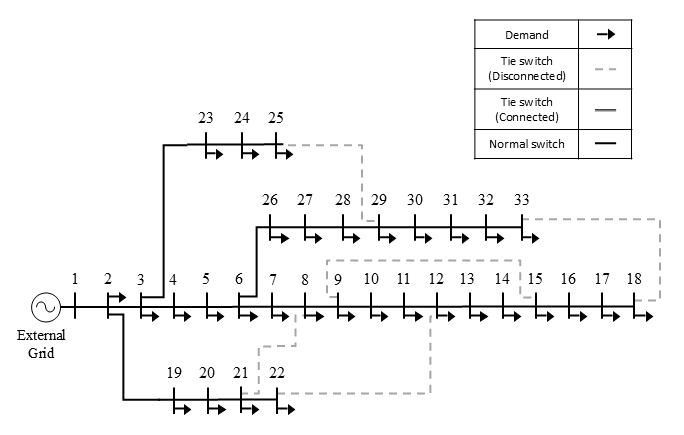
\includegraphics[width=4 in,keepaspectratio]{modified_33_bus_disc.png}
	\end{figure}

	
\end{frame}

%------------------------------------------------


\begin{frame}
	\frametitle{33-bus distribution system}
	\framesubtitle{Input Data - Load}

	\begin{figure}
		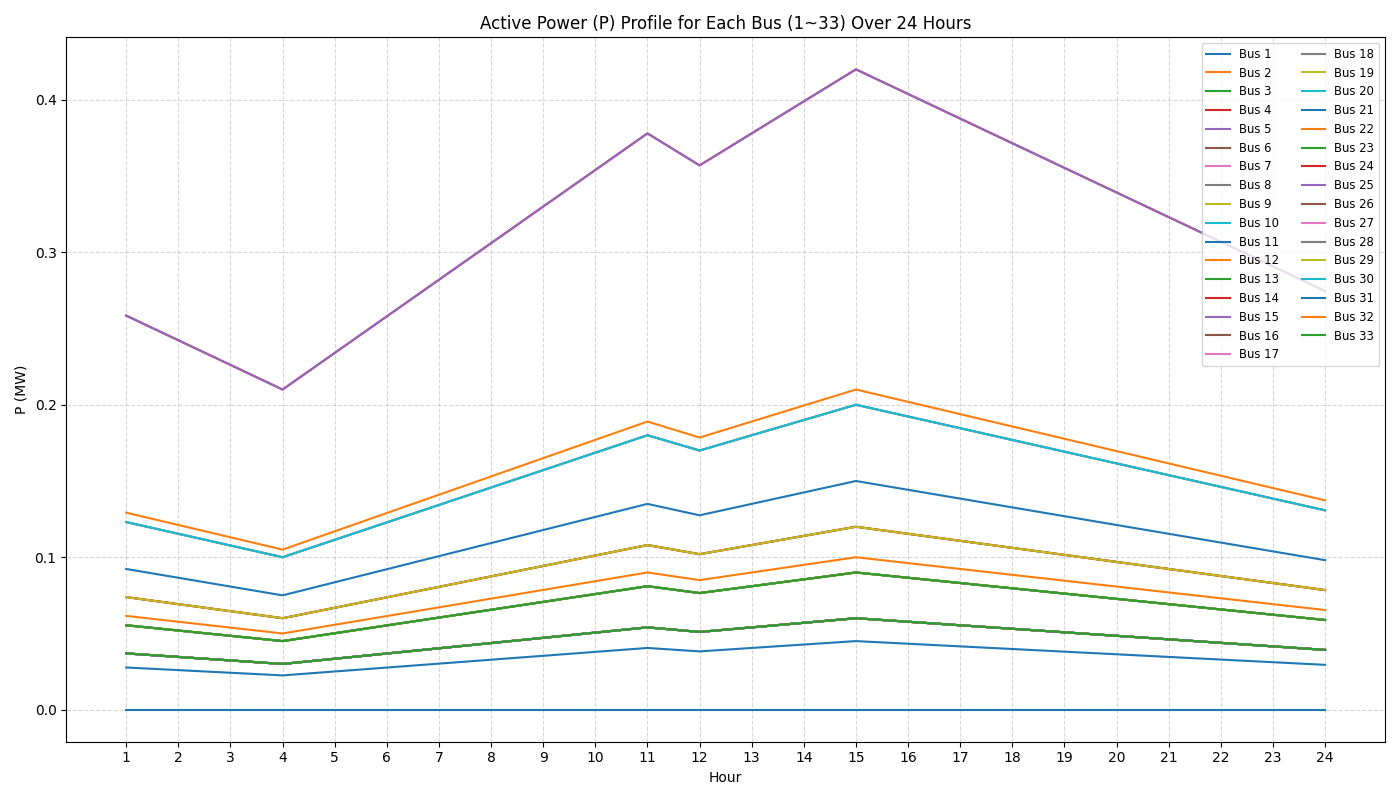
\includegraphics[width=3 in,keepaspectratio]{../fig/Load_P.png}
	\end{figure}

	\begin{itemize}
		\item The load data is based on the 24-hour load profile of a typical distribution system.
	\end{itemize}

	
\end{frame}

%------------------------------------------------

\begin{frame}
	\frametitle{33-bus distribution system}
	\framesubtitle{Input Data - Load}

	\begin{figure}
		\centering
		\begin{minipage}{0.16\textwidth}
			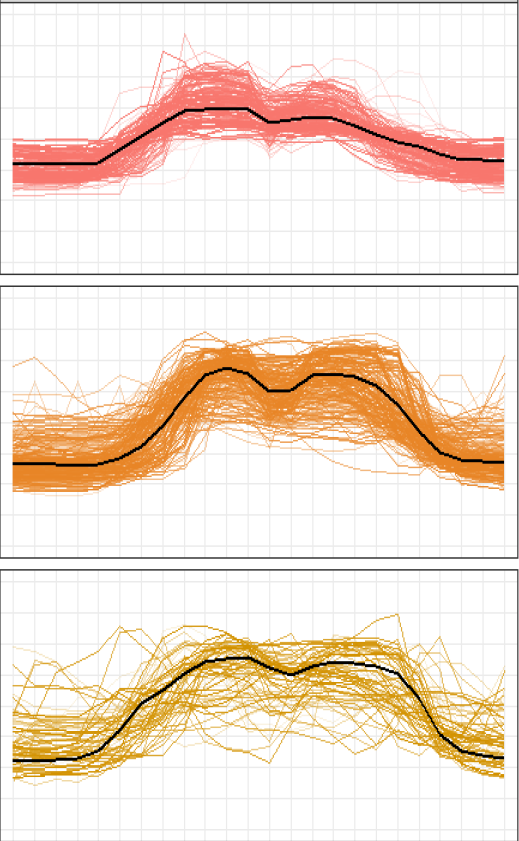
\includegraphics[width=\linewidth,keepaspectratio]{load_profile_1.png}
		\end{minipage}
		\begin{minipage}{0.16\textwidth}
			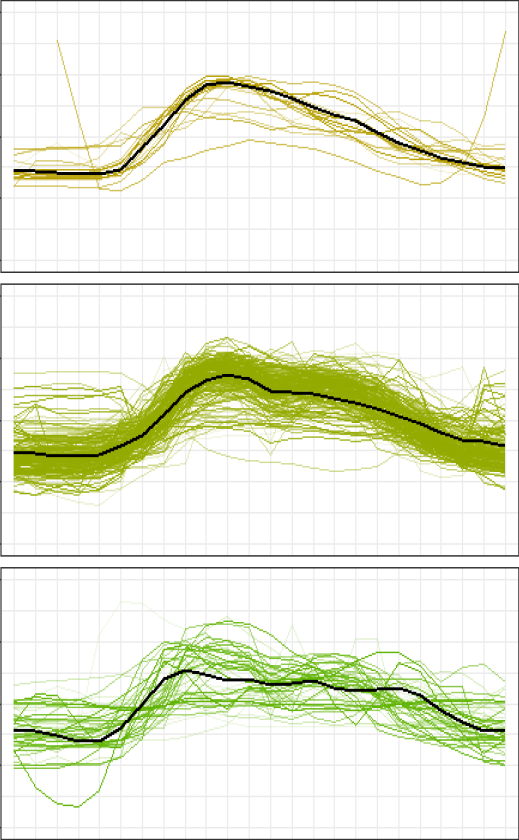
\includegraphics[width=\linewidth,keepaspectratio]{load_profile_2.png}
		\end{minipage}
		\begin{minipage}{0.16\textwidth}
			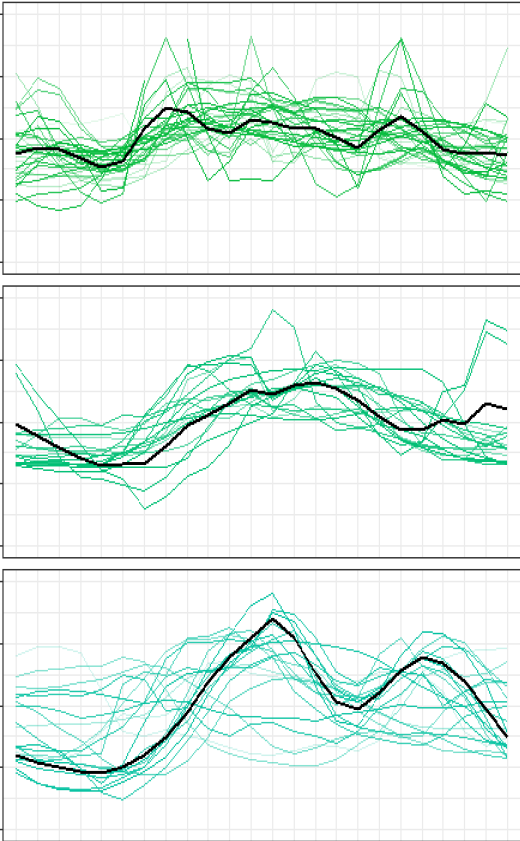
\includegraphics[width=\linewidth,keepaspectratio]{load_profile_3.png}
		\end{minipage}
		\begin{minipage}{0.16\textwidth}
			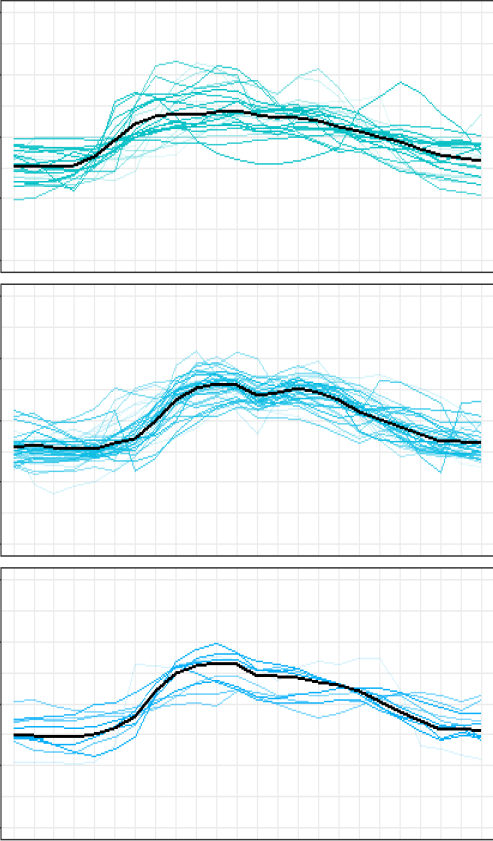
\includegraphics[width=\linewidth,keepaspectratio]{load_profile_4.png}
		\end{minipage}
		\begin{minipage}{0.16\textwidth}
			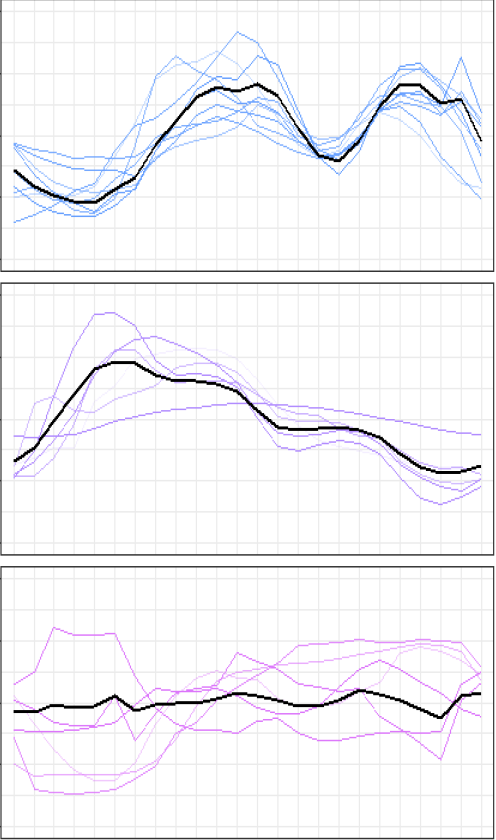
\includegraphics[width=\linewidth,keepaspectratio]{load_profile_5.png}
		\end{minipage}
		\begin{minipage}{0.16\textwidth}
			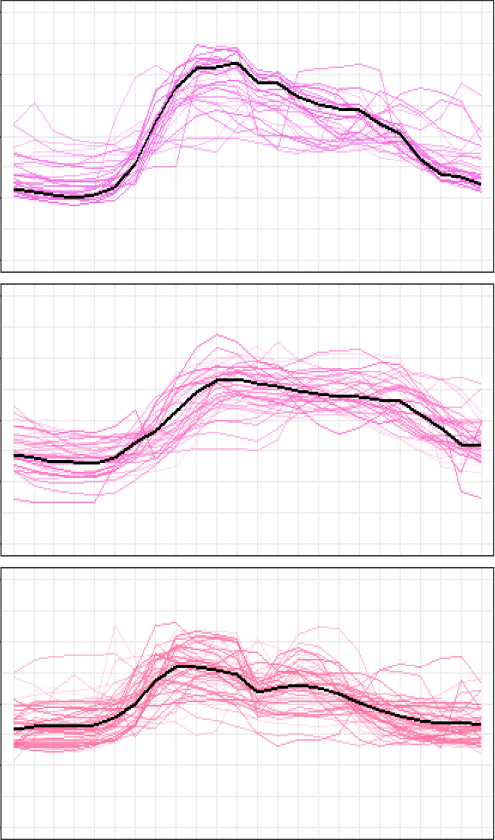
\includegraphics[width=\linewidth,keepaspectratio]{load_profile_6.png}
		\end{minipage}
	\end{figure}
	
	\begin{itemize}
		\item The 18 load patterns were randomly assigned to the existing 33-bus system.
	\end{itemize}
	\begin{quote}
		ELMAS: a one-year dataset of hourly electrical load profiles from 424 French industrial and tertiary sectors \ldots \parencite{Bellinguer2023}
	\end{quote}

\end{frame}

%------------------------------------------------


\begin{frame}
	\frametitle{33-bus distribution system}
	\framesubtitle{Output Data - Voltage magnitude}

	\begin{figure}
		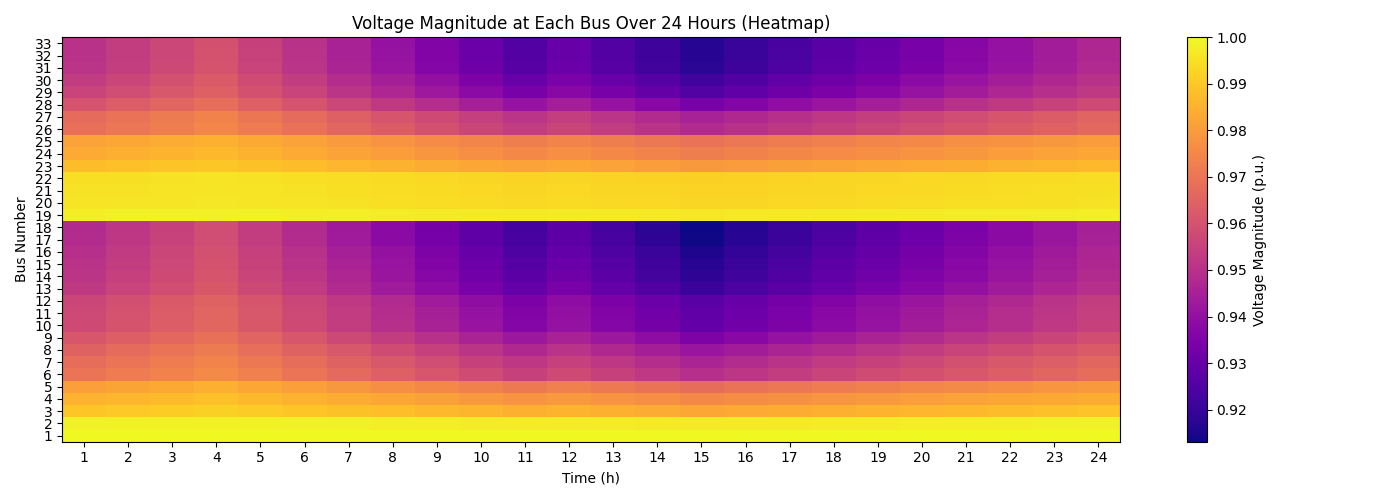
\includegraphics[width=5 in,keepaspectratio]{../fig/V_mag_heatmap.png}
	\end{figure}

	\begin{itemize}
		\item Increased demand leads to a larger voltage drop
		\item The voltage drop increases with distance from the generator(BUS 1).
	\end{itemize}

	
\end{frame}

%------------------------------------------------

\begin{frame}
	\frametitle{33-bus distribution system}
	\framesubtitle{Output Data - Voltage angle}

	\begin{figure}
		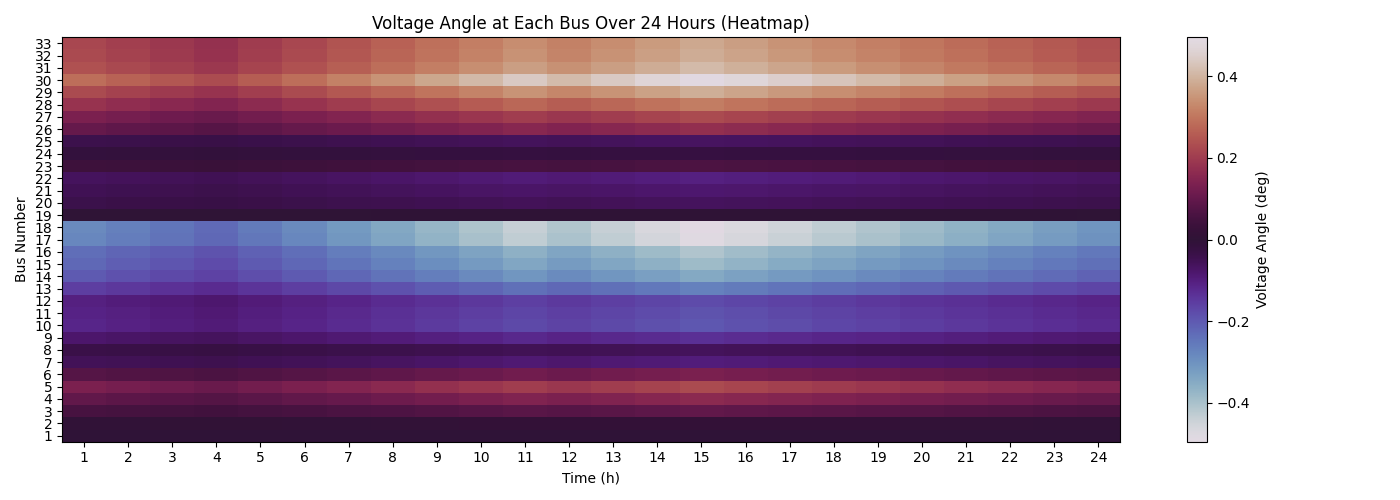
\includegraphics[width=5 in,keepaspectratio]{../fig/V_ang_heatmap.png}
	\end{figure}

		\begin{itemize}
		\item Increased demand leads to a greater phase angle.
		\item The phase angle tends to decrease with increasing distance from the generator.
		\item Bus 30 has a substantial reactive power demand.
	\end{itemize}

	
\end{frame}
%------------------------------------------------

\begin{frame}
	\frametitle{33-bus distribution system}
	\framesubtitle{Output Data - P line flow sending(at 13:00)}

	\begin{figure}
		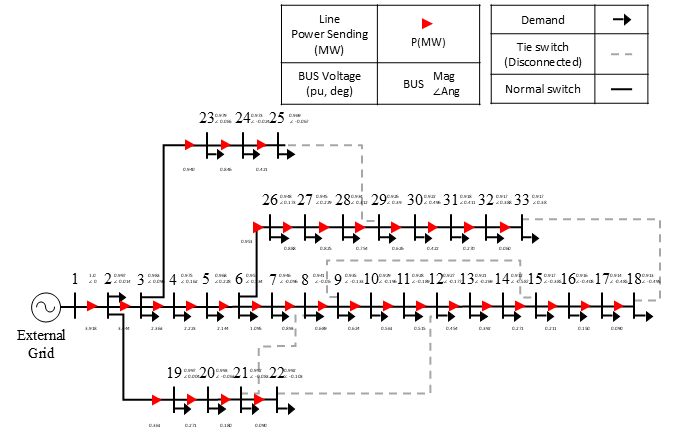
\includegraphics[width=4 in,keepaspectratio]{modified_33_bus_line_flow.png}
	\end{figure}

\end{frame}

%------------------------------------------------

% \subsection{Connected 33-bus distribution system}

% \begin{frame}
% 	\frametitle{Connected 33-bus distribution system}
% 	\framesubtitle{Structure of the Connected 33-bus distribution system}

% 	\begin{figure}
% 		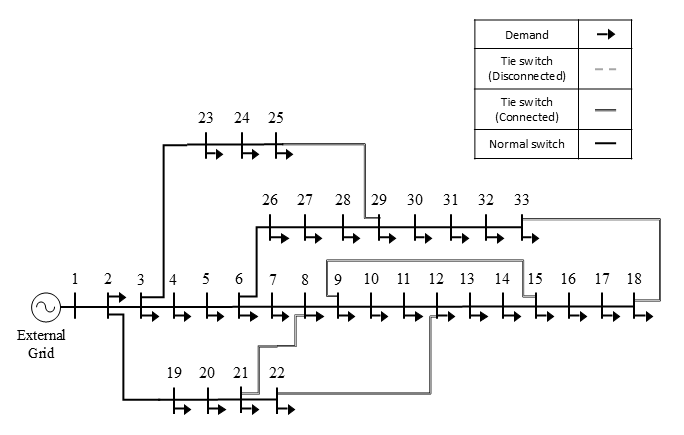
\includegraphics[width=4 in,keepaspectratio]{modified_33_bus_c.png}
% 	\end{figure}

	
% \end{frame}

%------------------------------------------------
\section{References}

%------------------------------------------------

\begin{frame} % Use [allowframebreaks] to allow automatic splitting across slides if the content is too long
	\frametitle{References}
	
	\printbibliography
	
	
\end{frame}


%----------------------------------------------------------------------------------------
%	ACKNOWLEDGMENTS SLIDE
%----------------------------------------------------------------------------------------

\begin{frame}
	\frametitle{Acknowledgements}
	
	\begin{columns}[t] % The "c" option specifies centered vertical alignment while the "t" option is used for top vertical alignment
		\begin{column}{0.45\textwidth} % Left column width
			\textbf{CWNU Power System Economis Lab}
			\begin{itemize}
				\item Woong Ko
				\item Taeho Nam
			\end{itemize}
			
		\end{column}		
		
	\end{columns}
\end{frame}

%----------------------------------------------------------------------------------------
%	CLOSING SLIDE
%----------------------------------------------------------------------------------------

\begin{frame}[plain] % The optional argument 'plain' hides the headline and footline
	\begin{center}
		{\Huge The End}
		
		\bigskip\bigskip % Vertical whitespace
		
		{\LARGE Questions? Comments?}
	\end{center}
\end{frame}

%----------------------------------------------------------------------------------------

\end{document} 